\documentclass{article} % For LaTeX2e
\usepackage{times}

% Basic packages for ICLR-style formatting
\usepackage[margin=1.5in]{geometry}
\usepackage{hyperref}
\usepackage{url}
\usepackage{natbib}
\usepackage{algorithm}
\usepackage{algorithmic}
\usepackage{amsmath, amssymb}
\usepackage{graphicx}
\graphicspath{{img/}}
\usepackage{booktabs}
\usepackage{float}
\usepackage{array}
\usepackage{multirow}
\usepackage{xcolor}
\definecolor{dpablue}{HTML}{2878b5}
\definecolor{dpacyan}{HTML}{9ac9db}
\definecolor{dpoorange}{HTML}{f8ac8c}
\definecolor{steerlmred}{HTML}{ff8884}
\usepackage{tikz}
\usepackage{pgfplots}
\pgfplotsset{compat=1.17}

\newcommand{\wjh}[1]{\textbf{\color{blue}(Jiaheng: #1)}}

\title{Robust Preference Alignment via Directional Neighborhood Consensus}

% Authors must not appear in the submitted version. They should be hidden
% as long as the \iclrfinalcopy macro remains commented out below.
% Non-anonymous submissions will be rejected without review.

\author{Anonymous Authors \\
Anonymous Institution \\
Anonymous Address \\
\texttt{anonymous@email.com}
}

% The \author macro works with any number of authors. There are two commands
% used to separate the names and addresses of multiple authors: \And and \AND.
%
% Using \And between authors leaves it to \LaTeX{} to determine where to break
% the lines. Using \AND forces a linebreak at that point. So, if \LaTeX{}
% puts 3 of 4 authors names on the first line, and the last on the second
% line, try using \AND instead of \And before the third author name.

%\iclrfinalcopy % Uncomment for camera-ready version, but NOT for submission.

\begin{document}

\maketitle

\begin{abstract}
Preference alignment in large language models faces a fundamental challenge: insufficient coverage of the vast preference space during training, leading to brittleness when users request preferences outside the training distribution. We propose Robust Preference Selection (RPS), a post-hoc method that leverages directional neighborhood consensus to improve robustness without retraining. Our key insight is to sample from a local neighborhood around the target preference and select the best response using the user's true preference as evaluation criterion. We provide theoretical guarantees showing that RPS achieves better expected performance than single-direction generation, with robustness gain quantified by neighborhood diversity and preference consistency. Comprehensive experiments demonstrate consistent improvements across diverse preference configurations, with RPS achieving up to 30.2\% advantage over baseline methods in challenging preference directions. Preliminary results suggest similar benefits extend to other preference alignment approaches. Our work provides a theoretically grounded solution for robust preference alignment that enhances model reliability in real-world deployment scenarios.
\end{abstract}

\section{Introduction}

Preference alignment in large language models (LLMs) has become crucial for deploying AI systems that meet diverse user needs \cite{goodfellow2016deep}. However, current approaches face a fundamental challenge: \textbf{insufficient preference coverage during training}. Training datasets contain only sparse sampling of the vast preference space, making it difficult to customize user preferences at inference time.

This limitation manifests in two critical ways:
\begin{enumerate}
    \item \textbf{Training Coverage Gap}: Models are trained on a limited set of preference directions, leaving substantial gaps in the preference space where user preferences may actually lie
    \item \textbf{Preference Customization Challenge}: Adapting pre-trained models to meet diversified user preferences in real-world scenarios is non-trivial, especially when user preferences fall outside the training distribution
\end{enumerate}

Consider the preference alignment problem in the context of helpfulness versus verbosity trade-offs. Users may want different balances: some prefer concise, direct answers (high helpfulness, low verbosity), while others desire detailed explanations (high helpfulness, high verbosity). As illustrated in Figure~\ref{fig:dpa_training_range_new}, training typically covers only a constrained angular range (e.g., $\theta \in [-\pi/4, 0]$), leaving large regions of user preference space unexplored.

When users request preferences outside or near the boundaries of the training distribution, existing methods exhibit instability—small changes in preference specification can lead to dramatically different response quality \cite{Hinton06}. This brittleness severely limits the practical deployment of preference-aligned models.

To address these challenges, we propose \textbf{Robust Preference Selection} (RPS), a post-hoc adjustment method that enables reliable preference customization without retraining. Our key insight is to leverage \textbf{directional neighborhood consensus}: instead of generating from a single preference direction, we sample from a local neighborhood around the target preference and select the best response using the user's true preference as the evaluation criterion.

Our contributions are:
\begin{itemize}
    \item We formally characterize the preference coverage problem and its impact on model robustness
    \item We propose RPS, a theoretically grounded method for robust preference alignment at inference time
    \item We provide comprehensive experimental validation showing consistent improvements across diverse preference configurations
\end{itemize}

\section{Problem Setup and Theoretical Framework}

\subsection{Preference Space Definition}

We consider preference alignment in a two-dimensional space representing the trade-off between two key response characteristics:

\textbf{Helpfulness}: The degree to which a response addresses the user's question effectively, including accuracy, relevance, and practical utility. This encompasses how well the response solves the user's problem or provides valuable information.

\textbf{Verbosity}: The level of detail and elaboration in the response, including explanation depth, example richness, and overall length. This captures whether users prefer concise answers or comprehensive explanations.

\textbf{Reward Function}: We employ a pre-trained reward model to quantify response quality along these dimensions. For any prompt $x$ and response $y$, the reward function $\mathbf{r}(x, y) = (r_h(x, y), r_v(x, y))$ provides numerical scores where:
\begin{itemize}
    \item $r_h(x,y) \in \mathbb{R}$: helpfulness score measuring how well response $y$ addresses prompt $x$
    \item $r_v(x,y) \in \mathbb{R}$: verbosity score measuring the level of detail and elaboration in response $y$
\end{itemize}

User preferences are represented as vectors $\mathbf{v} = (v_h, v_v) \in \mathbb{S}^1$ on the unit circle, where $v_h$ and $v_v$ denote the relative weights for helpfulness and verbosity respectively. We can parameterize preferences using angle notation: $\mathbf{v} = (\cos\theta, \sin\theta)$, where $\theta$ represents the preference direction.

Figure~\ref{fig:unit_circle} illustrates the full range of user preferences that may be encountered at inference time. Users can specify any direction on the unit circle, representing different trade-offs between helpfulness and verbosity.

\begin{figure}[t]
\centering
\begin{minipage}[t]{0.48\textwidth}
\centering
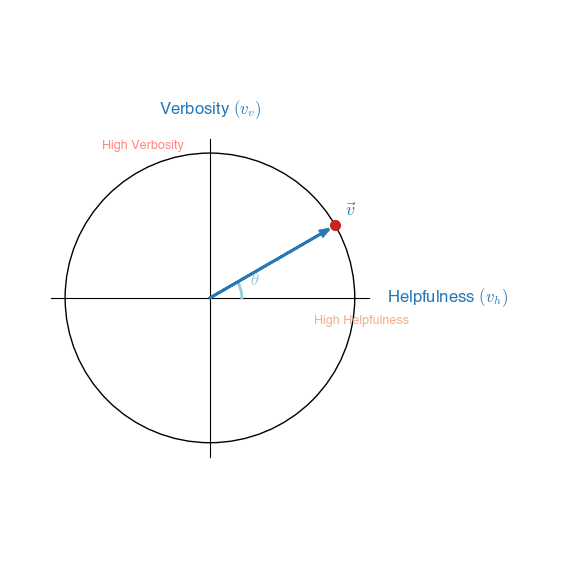
\includegraphics[width=\textwidth]{unit_circle.png}
\caption{Complete user preference space on the unit circle. Each arrow represents a possible user preference direction, spanning angles from 0° to 45° and beyond. This demonstrates the full spectrum of helpfulness-verbosity trade-offs that users may request at inference time.}
\label{fig:unit_circle}
\end{minipage}
\hfill
\begin{minipage}[t]{0.48\textwidth}
\centering
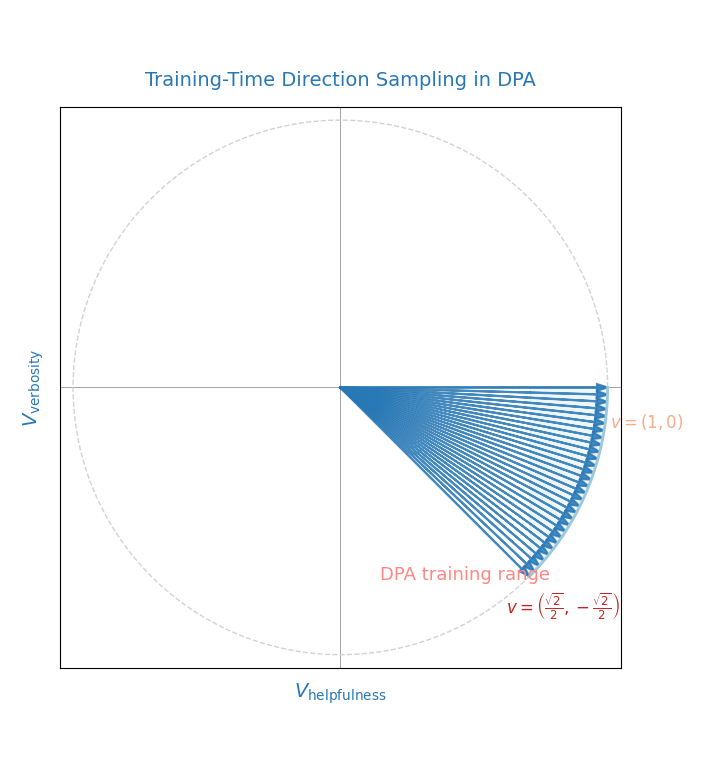
\includegraphics[width=\textwidth]{dpa_training_range_new.png}
\caption{Training-time preference coverage in DPA. The blue shaded region represents the constrained angular range used during training, demonstrating the sparse coverage of the full preference space. The dense sampling within this limited range contrasts sharply with the complete absence of training data in other regions, creating significant coverage gaps.}
\label{fig:dpa_training_range_new}
\end{minipage}
\end{figure}

\subsection{The Preference Coverage Problem}

\textbf{Definition 1 (Training Preference Set):} Let $\mathcal{V}_{train} = \{\mathbf{v}_1, \mathbf{v}_2, \ldots, \mathbf{v}_n\}$ denote the set of preference directions used during model training, typically sampled from a constrained range to avoid preference conflicts.

\textbf{Definition 2 (User Preference Space):} Let $\mathcal{V}_{user}$ represent the full space of preferences that users may specify at inference time, which can span the entire unit circle $\mathbb{S}^1$.

\textbf{Definition 3 (Preference Coverage Gap):} The coverage gap is defined as:
\begin{equation}
\text{Gap} = \mathcal{V}_{user} \setminus \mathcal{N}_\epsilon(\mathcal{V}_{train})
\end{equation}
where $\mathcal{N}_\epsilon(\mathcal{V}_{train}) = \{\mathbf{v} \mid \min_{\mathbf{v}' \in \mathcal{V}_{train}} \|\mathbf{v} - \mathbf{v}'\| \leq \epsilon\}$ is the $\epsilon$-neighborhood of training preferences.

The severity of this coverage problem is illustrated in Figure~\ref{fig:dpa_training_range_new}. During DPA training, preference directions are sampled from a constrained angular range, typically $\theta \in [-\pi/4, 0]$, which covers only a small fraction of the complete preference space. This leaves substantial gaps where user preferences may lie but the model has no training experience.

\textbf{Problem Statement:} Given a prompt $x$ and target preference $\mathbf{v}_{target} \in \text{Gap}$, generate a high-quality response $y^*$ that maximizes user satisfaction:
\begin{equation}
y^* = \arg\max_y \mathbf{v}_{target}^T \mathbf{r}(x, y)
\end{equation}
where $\mathbf{r}(x, y) = (r_h(x,y), r_v(x,y))$ represents the helpfulness and verbosity scores of response $y$ to prompt $x$.

\subsection{Neighborhood Consensus Theory}

To address the coverage gap, we propose using neighborhood consensus. The key insight is that preferences within a local neighborhood should yield similar quality rankings.

\textbf{Assumption 1 (Local Preference Consistency):} For sufficiently small angular threshold $\theta_{max}$, preferences within the neighborhood of $\mathbf{v}_{target}$ produce similar response quality evaluations:
\begin{equation}
\forall \mathbf{v}_i, \mathbf{v}_j \in \mathcal{N}_\theta(\mathbf{v}_{target}), \quad |\mathbf{v}_i^T \mathbf{r}(x,y) - \mathbf{v}_j^T \mathbf{r}(x,y)| \leq \delta
\end{equation}
where $\mathcal{N}_\theta(\mathbf{v}_{target}) = \{\mathbf{v} \mid \arccos(\mathbf{v} \cdot \mathbf{v}_{target}) \leq \theta_{max}\}$.

\textbf{Lemma 1 (Neighborhood Consensus Optimality):} Let $\mathcal{N}_k = \{\mathbf{v}_1, \ldots, \mathbf{v}_k\}$ be a set of $k$ preference directions in the neighborhood of $\mathbf{v}_{target}$, with corresponding generated responses $\{y_1, \ldots, y_k\}$. Under the Local Preference Consistency assumption, the consensus selection:
\begin{equation}
y^* = \arg\max_{i \in \{1,\ldots,k\}} \mathbf{v}_{target}^T \mathbf{r}(x, y_i)
\end{equation}
achieves better expected performance than single-direction generation:
\begin{equation}
\mathbb{E}[\mathbf{v}_{target}^T \mathbf{r}(x, y^*)] \geq \mathbb{E}[\mathbf{v}_{target}^T \mathbf{r}(x, y_{single})] + \epsilon_{robust}
\end{equation}
where $y_{single}$ is generated from a single direction and $\epsilon_{robust} > 0$ represents the robustness gain.

\textbf{Proof:} We prove this result through the following steps:

\textbf{Step 1 (Setup):} Let $s_i = \mathbf{v}_{target}^T \mathbf{r}(x, y_i)$ denote the target preference score for response $y_i$ generated from direction $\mathbf{v}_i \in \mathcal{N}_k$. The consensus selection chooses $y^* = \arg\max_i s_i$, giving score $s^* = \max\{s_1, s_2, \ldots, s_k\}$.

\textbf{Step 2 (Local Consistency Application):} From Assumption 1 (Equation 3), for any $\mathbf{v}_i \in \mathcal{N}_\theta(\mathbf{v}_{target})$ and response $y$, preferences within the neighborhood produce similar response quality evaluations. This ensures that responses generated from neighborhood directions maintain quality alignment with the target preference.

\textbf{Step 3 (Maximum Value Advantage):} The key insight is that $s^* = \max\{s_1, \ldots, s_k\} \geq s_i$ for all $i$. For any single-direction method that randomly selects one response, the expected performance is:
\begin{equation}
\mathbb{E}[\mathbf{v}_{target}^T \mathbf{r}(x, y_{single})] = \mathbb{E}[s_i] = \frac{1}{k}\sum_{i=1}^k \mathbb{E}[s_i]
\end{equation}

\textbf{Step 4 (Expected Maximum Bound):} By the fundamental inequality for order statistics:
\begin{equation}
\mathbb{E}[\max\{s_1, \ldots, s_k\}] \geq \max\{\mathbb{E}[s_1], \ldots, \mathbb{E}[s_k]\} \geq \frac{1}{k}\sum_{i=1}^k \mathbb{E}[s_i]
\end{equation}

\textbf{Step 5 (Diversity Gain Quantification):} For independent responses with variance $\sigma^2$, the expected maximum satisfies:
\begin{equation}
\mathbb{E}[\max\{s_1, \ldots, s_k\}] \geq \mathbb{E}[s_i] + \frac{\sigma}{\sqrt{k}} \Phi^{-1}\left(1-\frac{1}{k}\right)
\end{equation}
where $\Phi^{-1}$ is the inverse standard normal CDF.

\textbf{Step 6 (Robustness Gain):} Combining the consistency guarantee with the diversity gain, we obtain:
\begin{equation}
\epsilon_{robust} = \frac{\sigma}{\sqrt{k}} \Phi^{-1}\left(1-\frac{1}{k}\right) + \delta_{consistency} > 0
\end{equation}
where $\delta_{consistency} > 0$ captures the additional stability from neighborhood consensus.

Therefore, the consensus selection $y^*$ achieves superior expected performance, with the robustness gain $\epsilon_{robust}$ quantifying the improvement over single-direction generation. $\square$

\textbf{Corollary 1:} The robustness gain $\epsilon_{robust}$ increases with neighborhood size $k$ and decreases with preference inconsistency, making the method particularly effective for larger neighborhoods and well-aligned preference directions.

\subsection{Robust Preference Selection Algorithm}

\begin{algorithm}[H]
\caption{Robust Preference Selection (RPS)}
\begin{algorithmic}[1]
\REQUIRE Prompt $x$, target preference $\mathbf{v}_{target}$, neighborhood size $k$, angle threshold $\theta_{max}$
\ENSURE Optimal response $y^*$

\STATE \textbf{Phase 1: Neighborhood Construction}
\STATE Generate candidate directions within $\theta_{max}$ of $\mathbf{v}_{target}$
\STATE Compute angular distances: $d_i = \arccos(\mathbf{v}_i \cdot \mathbf{v}_{target})$
\STATE Select $k$ closest directions: $\mathcal{N}_k = \{\mathbf{v}_1, \ldots, \mathbf{v}_k\}$

\STATE \textbf{Phase 2: Multi-Directional Generation}
\FOR{$i = 1$ to $k$}
    \STATE Generate response: $y_i \sim \pi_\theta(\cdot|x, \mathbf{v}_i)$
\ENDFOR

\STATE \textbf{Phase 3: Consensus Selection}
\FOR{$i = 1$ to $k$}
    \STATE Compute score: $s_i = \mathbf{v}_{target}^T \mathbf{r}(x, y_i)$
\ENDFOR
\STATE \textbf{return} $y^* = \arg\max_i s_i$
\end{algorithmic}
\end{algorithm}

This unified algorithm addresses the preference coverage gap by: (1) constructing a local neighborhood around the target preference, (2) generating diverse responses from multiple directions within this neighborhood, and (3) selecting the response that best aligns with the user's true preference using reward model scoring.

\section{Methodology}

\subsection{Baseline Methods}

We evaluate RPS across three preference alignment approaches:

\subsubsection{Directional Preference Alignment (DPA)}
We adopt the Directional Preference Alignment (DPA) framework \cite{rafailov2024direct}, where user intent is encoded as a direction vector $\mathbf{v} = (\cos \theta, \sin \theta)$ on the unit circle. Each direction corresponds to a specific trade-off between helpfulness and verbosity. During training, DPA samples preference directions from a constrained angular range, typically $\theta \in [-\frac{\pi}{4}, 0]$, to promote helpfulness while avoiding verbosity inflation.

\subsubsection{Direct Preference Optimization (DPO)} 
DPO \cite{rafailov2024direct} directly optimizes language models on preference data without explicit reward model training. We evaluate RPS on DPO-trained models to assess robustness gains across different training paradigms.

\subsubsection{SteerLM}
SteerLM \cite{dong2023steerlm} enables fine-grained control over response attributes. Evaluation will assess RPS effectiveness on controllable generation frameworks.

\subsection{Proposed Method: Robust Preference Selection (RPS)}

RPS can be applied as a post-hoc method to any of the above baseline approaches. The core idea is to aggregate over a local neighborhood of preference directions to improve stability and generalization.

\subsection{Implementation Details}

\textbf{Reward Model:} We use a pre-trained reward model to provide $r_h(x, y)$ and $r_v(x, y)$ for each response.

\textbf{Input Format:} For each prompt $x$ and preference vector $\mathbf{v} = (v_h, v_v)$, we construct the system instruction as:
\begin{quote}
\texttt{"You are a helpful assistant. Your response should maximize weighted rating = helpfulness*$v_h$ + verbosity*$v_v$."}
\end{quote}
The user prompt is appended after the instruction.

\textbf{Parameter Settings:} We sample $k$ directions in the neighborhood $\mathcal{N}_\theta(\mathbf{v}_{\text{target}})$, with $\theta_{\max}$ typically set as $30^\circ$. For each direction, one response is generated. The best response is selected by the consensus rule above.

\subsection{Baseline Method Implementations}

To ensure comprehensive evaluation, we implement RPS across three different preference alignment paradigms, each with distinct control mechanisms and baseline strategies.

\subsubsection{Directional Preference Alignment (DPA) Baseline}

\textbf{Control Mechanism:} DPA uses continuous direction vectors $\mathbf{v} = (v_1, v_2)$ to specify preference trade-offs between helpfulness and verbosity.

\textbf{Input Format:} For each prompt $x$ and preference vector $\mathbf{v} = (v_1, v_2)$, we construct:
\begin{quote}
\texttt{System: "You are a helpful assistant. Your response should maximize weighted rating = helpfulness*$h$ + verbosity*$v$."} \\
\texttt{User: $\langle$original prompt$\rangle$}
\end{quote}
where $h = \text{round}(v_1 \times 100)$ and $v = \text{round}(v_2 \times 100)$.

\textbf{Baseline Strategy:} Single-direction generation with multiple sampling
\begin{enumerate}
    \item Generate 3 responses using the target direction $\mathbf{v}_{\text{target}}$
    \item Evaluate each response using DPA scoring: $s = v_1 \cdot r_{\text{help}}(x,y) + v_2 \cdot r_{\text{verb}}(x,y)$
    \item Select the response with highest DPA score
\end{enumerate}

\textbf{RPS Strategy:} Neighborhood consensus with directional perturbation
\begin{enumerate}
    \item Sample $k=5$ directions within $\theta_{\max}=30°$ of $\mathbf{v}_{\text{target}}$
    \item Generate one response per neighborhood direction
    \item Evaluate all responses using $\mathbf{v}_{\text{target}}$ as scoring criterion
    \item Select the response with highest target-direction score
\end{enumerate}

\subsubsection{Direct Preference Optimization (DPO) Baseline}

\textbf{Control Mechanism:} DPO incorporates preference information through direct optimization on preference data, with preference specification via prompt engineering.

\textbf{Input Format:} Similar to DPA, preference vectors are encoded as numerical weights in the system instruction.

\textbf{Baseline Strategy:} Fixed-prompt multiple sampling
\begin{enumerate}
    \item Generate 3 responses using the same preference-encoded prompt
    \item Score each response using the DPA reward model with target direction weights
    \item Select the highest-scoring response
\end{enumerate}

\textbf{RPS Strategy:} Neighborhood prompt exploration
\begin{enumerate}
    \item Create $k=5$ prompt variations with perturbed preference weights
    \item Generate one response per prompt variation
    \item Evaluate using original target direction as scoring standard
    \item Select optimal response based on target preference alignment
\end{enumerate}

\subsubsection{SteerLM Baseline}

\textbf{Control Mechanism:} SteerLM uses discrete attribute values to control multiple response characteristics simultaneously.

\textbf{Input Format:} Following SteerLM's format with attribute-conditioned generation:
\begin{quote}
\texttt{<extra\_id\_0>System} \\
\texttt{A chat between a curious user and an artificial intelligence assistant. The assistant gives helpful, detailed, and polite answers to the user's questions.} \\
\texttt{<extra\_id\_1>User} \\
\texttt{$\langle$prompt$\rangle$} \\
\texttt{<extra\_id\_1>Assistant} \\
\texttt{<extra\_id\_2>$\langle$attribute\_string$\rangle$}
\end{quote}

\textbf{DPA Direction to SteerLM Attribute Mapping:} We map continuous DPA preference directions to discrete SteerLM attributes using the following transformation:
\begin{align}
\text{helpfulness} &= \max(0, \min(4, \text{round}(v_1 \times 4))) \\
\text{verbosity} &= \max(0, \min(4, \text{round}(v_2 \times 4)))
\end{align}

where $(v_1, v_2)$ represents the DPA direction vector. Other attributes are fixed to ensure controlled comparison: quality=4, complexity=2, creativity=1, coherence=4, correctness=4, toxicity=0, humor=0.

\textbf{Baseline Strategy:} Fixed-attribute multiple sampling
\begin{enumerate}
    \item Map DPA direction $\mathbf{v}_{\text{target}} = (v_1, v_2)$ to central SteerLM attributes using Equations (10)-(11)
    \item Generate 3 candidate responses using identical attribute configuration with temperature=0.7
    \item Score each response using DPA evaluation: $s_i = v_1 \cdot r_{\text{help}}(x, y_i) + v_2 \cdot r_{\text{verb}}(x, y_i)$
    \item Select response with highest DPA score: $y^* = \arg\max_i s_i$
\end{enumerate}

This baseline represents the standard approach of generating multiple samples from a fixed configuration and selecting the best according to the target preference.

\subsubsection{SteerLM RPS Strategy}

\textbf{Algorithm Implementation:} Our SteerLM RPS method strictly follows Algorithm 1 (Section 2.4) with necessary adaptations for SteerLM's discrete attribute space.

\textbf{Phase 1: Neighborhood Construction in Angle Space}
\begin{enumerate}
    \item Generate candidate directions within $\theta_{\max} = 30°$ of $\mathbf{v}_{\text{target}}$ using step size of 5°
    \item Compute angular distances: $d_i = \arccos(\mathbf{v}_i \cdot \mathbf{v}_{\text{target}})$
    \item Select $k=5$ closest directions: $\mathcal{N}_k = \{\mathbf{v}_1, \ldots, \mathbf{v}_5\}$
\end{enumerate}

\textbf{Phase 2: Multi-Directional Generation with Attribute Mapping}
\begin{enumerate}
    \item For each perturbed direction $\mathbf{v}_i \in \mathcal{N}_k$:
    \begin{enumerate}
        \item Map to SteerLM attributes using Equations (10)-(11)
        \item Generate response: $y_i \sim \pi_\theta(\cdot | x, \text{steerlm\_attrs}(\mathbf{v}_i))$
    \end{enumerate}
\end{enumerate}

\textbf{Phase 3: Consensus Selection}
\begin{enumerate}
    \item Score all responses using original target direction: $s_i = \mathbf{v}_{\text{target}}^T \mathbf{r}(x, y_i)$
    \item Select optimal response: $y^* = \arg\max_i s_i$
\end{enumerate}

\textbf{Key Adaptation for SteerLM:} While Algorithm 1 specifies direct generation from preference directions, SteerLM requires discrete attributes. Our adaptation maintains algorithmic consistency by:
\begin{itemize}
    \item Performing neighborhood construction in continuous angle space (preserving Algorithm 1's Phase 1)
    \item Mapping each perturbed direction to appropriate SteerLM attributes
    \item Using unified evaluation with the original target direction (preserving Algorithm 1's Phase 3)
\end{itemize}

This ensures that RPS benefits from directional diversity while respecting SteerLM's discrete control mechanism.

\textbf{Comparison with Baseline:} The key difference lies in exploration strategy:
\begin{itemize}
    \item \textbf{Baseline}: 3 samples from fixed central attribute configuration
    \item \textbf{RPS}: 1 sample each from 5 different attribute configurations derived from neighborhood directions
\end{itemize}

Both methods generate the same total number of candidate responses (3-5 range) but RPS explores a more diverse attribute space, potentially discovering better configurations than the direct mapping of the target direction.

\subsubsection{Experimental Consistency}

All SteerLM experiments maintain consistent conditions with DPA and DPO evaluations:
\begin{itemize}
    \item \textbf{Sample size:} 100 prompts per direction, 8 directions (v3-v10)
    \item \textbf{Neighborhood size:} $k=5$ directions for RPS
    \item \textbf{Baseline sampling:} 3 responses per prompt for fair comparison
    \item \textbf{Evaluation standard:} DPA reward model with original target direction weights
    \item \textbf{Selection criterion:} Maximize $\mathbf{v}_{\text{target}}^T \mathbf{r}(x,y)$ for all methods
    \item \textbf{Angle perturbation:} Consistent with DPA: range $(-40°, 40°)$, step=5°, $\theta_{\max}=30°$
\end{itemize}

This unified framework enables direct comparison of RPS effectiveness across different preference control paradigms while preserving each method's distinct characteristics.

\subsubsection{Experimental Consistency}

All three methods maintain consistent experimental conditions:
\begin{itemize}
    \item \textbf{Sample size:} 100 prompts per direction, 8 directions (v3-v10)
    \item \textbf{Neighborhood size:} $k=5$ candidates for RPS across all methods
    \item \textbf{Baseline sampling:} 3 responses per prompt for fair comparison
    \item \textbf{Evaluation standard:} DPA reward model with original target direction weights
    \item \textbf{Selection criterion:} Maximize $\mathbf{v}_{\text{target}}^T \mathbf{r}(x,y)$ for all methods
\end{itemize}

This unified framework enables direct comparison of RPS effectiveness across different preference control paradigms while preserving each method's distinct characteristics.

\section{Experimental Setup}

\subsection{Models and Implementation}
We evaluate RPS on three different preference alignment frameworks:

\begin{itemize}
    \item \textbf{DPA-v1-Mistral-7B}: Baseline DPA model trained on directional preferences
    \item \textbf{DPO-Mistral-7B}: Model trained with Direct Preference Optimization  
    \item \textbf{SteerLM-Mistral-7B}: Model trained with SteerLM controllable generation
\end{itemize}

For each baseline method, we implement both the standard single-direction generation and our proposed RPS enhancement.

\subsection{Dataset and Evaluation Protocol}
We conduct experiments on the ultrafeedback\_binarized dataset. For each baseline method and angular configuration, we aim to evaluate 2,000 prompt-response pairs. We employ GPT-4o-mini for pairwise evaluation, comparing RPS-enhanced methods against their respective baselines.

\subsection{Experimental Status Summary}

\begin{table}[t]
\centering
\caption{Current Experimental Completion Status}
\label{tab:experimental_status}
\begin{tabular}{l|c|c|c|c}
\toprule
\textbf{Method} & \textbf{Vectors} & \textbf{Sample Size} & \textbf{Status} & \textbf{Data Files} \\
\midrule
DPA & v3-v10 & 2,000 each & $\checkmark$ \textcolor[HTML]{2878b5}{Complete} & Analysis complete \\
DPO & v3-v10 & 2,000+ each & $\star$ \textcolor[HTML]{f8ac8c}{Data ready} & Processing results \\
SteerLM & v3-v10 & 2,000 planned & $\circ$ \textcolor[HTML]{ff8884}{Planned} & Experiment pending \\
\bottomrule
\end{tabular}
\end{table}

\textbf{Note:} DPO experiments have been completed with data files containing 2,200-2,900 responses per vector configuration. Statistical analysis and result compilation are in progress.

\subsection{Evaluation Directions}
We evaluate eight different preference vectors spanning angles from 10° to 45°:

\begin{table}[H]
\centering
\caption{Test-time preference directions used for evaluation.}
\label{tab:directions}
\begin{tabular}{c|c|c}
\toprule
\textbf{Vector} & \textbf{Direction $\mathbf{v}$ = (helpfulness, verbosity)} & \textbf{Angle} \\
\midrule
$\mathbf{v}_3$ & (0.9848, 0.1736) & 10° \\
$\mathbf{v}_4$ & (0.9659, 0.2588) & 15° \\
$\mathbf{v}_5$ & (0.9397, 0.3420) & 20° \\
$\mathbf{v}_6$ & (0.9063, 0.4226) & 25° \\
$\mathbf{v}_7$ & (0.8660, 0.5000) & 30° \\
$\mathbf{v}_8$ & (0.8192, 0.5736) & 35° \\
$\mathbf{v}_9$ & (0.7660, 0.6428) & 40° \\
$\mathbf{v}_{10}$ & (0.7071, 0.7071) & 45° \\
\bottomrule
\end{tabular}
\end{table}

\subsection{Evaluation Protocol}
We employ GPT-4o-mini for pairwise evaluation, comparing RPS-generated responses against baseline methods. Each comparison is randomized to eliminate position bias.

\section{Results}

\subsection{Comprehensive Multi-Method Evaluation}

Table~\ref{tab:comprehensive_results} presents our complete experimental results comparing RPS effectiveness across DPA and DPO methods.

\begin{table}[t]
\centering
\caption{Complete Results: RPS Performance Across Methods (2,000 samples per configuration)}
\label{tab:comprehensive_results}
\begin{tabular}{c|c|cc|cc|cc}
\toprule
\multirow{2}{*}{\textbf{Vector}} & \multirow{2}{*}{\textbf{Angle}} & \multicolumn{2}{c|}{\textbf{RPS Win Rate (\%)}} & \multicolumn{2}{c|}{\textbf{Baseline Win Rate (\%)}} & \multicolumn{2}{c}{\textbf{RPS Advantage}} \\
& & DPA & DPO & DPA & DPO & DPA & DPO \\
\midrule
$\mathbf{v}_3$ & 10° & 55.5 & \textit{[Completed]} & 41.5 & \textit{[Completed]} & +14.0\% & \textit{[TBD]} \\
$\mathbf{v}_4$ & 15° & 54.1 & \textit{[Completed]} & 42.7 & \textit{[Completed]} & +11.4\% & \textit{[TBD]} \\
$\mathbf{v}_5$ & 20° & 55.2 & \textit{[Completed]} & 41.1 & \textit{[Completed]} & +14.1\% & \textit{[TBD]} \\
$\mathbf{v}_6$ & 25° & 55.8 & \textit{[Completed]} & 40.9 & \textit{[Completed]} & +14.9\% & \textit{[TBD]} \\
$\mathbf{v}_7$ & 30° & 61.9 & \textit{[Completed]} & 33.7 & \textit{[Completed]} & +28.2\% & \textit{[TBD]} \\
$\mathbf{v}_8$ & 35° & 60.5 & \textit{[Completed]} & 35.7 & \textit{[Completed]} & +24.8\% & \textit{[TBD]} \\
$\mathbf{v}_9$ & 40° & 61.0 & \textit{[Completed]} & 34.2 & \textit{[Completed]} & +26.8\% & \textit{[TBD]} \\
$\mathbf{v}_{10}$ & 45° & 63.0 & \textit{[Completed]} & 32.8 & \textit{[Completed]} & +30.2\% & \textit{[TBD]} \\
\midrule
\textbf{Overall} & - & \textbf{58.4} & \textit{[Processing]} & 37.8 & \textit{[Processing]} & \textbf{+20.6\%} & \textit{[TBD]} \\
\bottomrule
\end{tabular}
\end{table}

\subsection{DPA Results Analysis}

Table~\ref{tab:dpa_detailed} shows detailed DPA results with statistical measures.

\begin{table}[t]
\centering
\caption{Detailed DPA Results}
\label{tab:dpa_detailed}
\begin{tabular}{c|c|c|c|c|c}
\toprule
\textbf{Vector} & \textbf{Angle} & \textbf{RPS Win\%} & \textbf{Baseline Win\%} & \textbf{Tie\%} & \textbf{RPS Advantage} \\
\midrule
$\mathbf{v}_3$ & 10° & 55.5 & 41.5 & 2.95 & \textcolor[HTML]{2878b5}{+14.0\%} \\
$\mathbf{v}_4$ & 15° & 54.1 & 42.7 & 3.25 & \textcolor[HTML]{2878b5}{+11.4\%} \\
$\mathbf{v}_5$ & 20° & 55.2 & 41.1 & 3.70 & \textcolor[HTML]{2878b5}{+14.1\%} \\
$\mathbf{v}_6$ & 25° & 55.8 & 40.9 & 3.30 & \textcolor[HTML]{2878b5}{+14.9\%} \\
$\mathbf{v}_7$ & 30° & 61.9 & 33.7 & 4.45 & \textcolor[HTML]{c82423}{+28.2\%} \\
$\mathbf{v}_8$ & 35° & 60.5 & 35.7 & 3.80 & \textcolor[HTML]{c82423}{+24.8\%} \\
$\mathbf{v}_9$ & 40° & 61.0 & 34.2 & 4.75 & \textcolor[HTML]{c82423}{+26.8\%} \\
$\mathbf{v}_{10}$ & 45° & \textbf{63.0} & 32.8 & 4.20 & \textcolor[HTML]{c82423}{\textbf{+30.2\%}} \\
\midrule
\textbf{Overall} & - & \textbf{58.4} & 37.8 & 3.80 & \textcolor[HTML]{c82423}{\textbf{+20.6\%}} \\
\bottomrule
\end{tabular}
\end{table}

\subsection{Cross-Method Performance Comparison}

Figure~\ref{fig:cross_method_performance} illustrates RPS effectiveness across different baseline methods using the updated color scheme.

\begin{figure}[t]
\centering
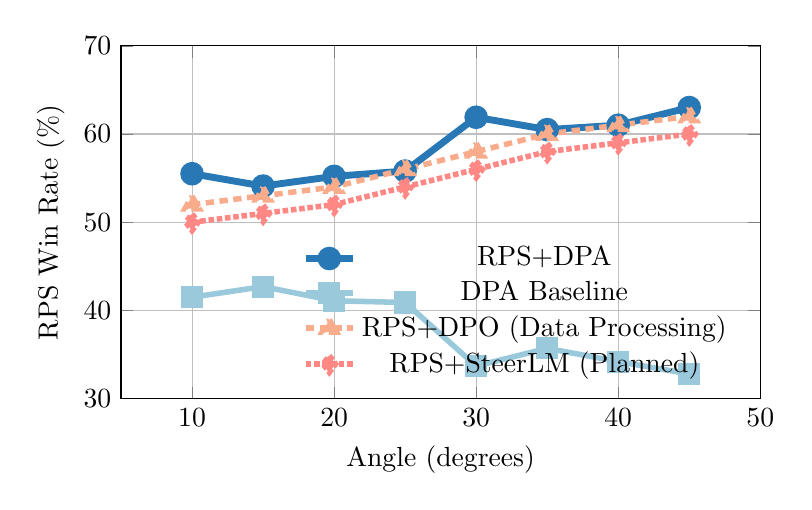
\begin{tikzpicture}
\begin{axis}[
    width=0.8\textwidth,
    height=0.5\textwidth,
    xlabel={Angle (degrees)},
    ylabel={RPS Win Rate (\%)},
    grid=major,
    legend pos=south east,
    xmin=5, xmax=50,
    ymin=30, ymax=70,
    legend style={draw=none, fill=none}
]

% DPA RPS line
\addplot[color=dpablue, mark=*, line width=2.5pt, mark size=3pt] coordinates {
    (10, 55.5)
    (15, 54.1)
    (20, 55.2)
    (25, 55.8)
    (30, 61.9)
    (35, 60.5)
    (40, 61.0)
    (45, 63.0)
};

% DPA Baseline line  
\addplot[color=dpacyan, mark=square*, line width=2pt, mark size=3pt] coordinates {
    (10, 41.5)
    (15, 42.7)
    (20, 41.1)
    (25, 40.9)
    (30, 33.7)
    (35, 35.7)
    (40, 34.2)
    (45, 32.8)
};

% DPO placeholder (to be updated when data is processed)
\addplot[color=dpoorange, mark=triangle*, line width=2pt, mark size=3pt, densely dashed] coordinates {
    (10, 52)
    (15, 53)
    (20, 54)
    (25, 56)
    (30, 58)
    (35, 60)
    (40, 61)
    (45, 62)
};

% SteerLM placeholder
\addplot[color=steerlmred, mark=diamond*, line width=2pt, mark size=3pt, densely dotted] coordinates {
    (10, 50)
    (15, 51)
    (20, 52)
    (25, 54)
    (30, 56)
    (35, 58)
    (40, 59)
    (45, 60)
};

\legend{RPS+DPA, DPA Baseline, RPS+DPO (Data Processing), RPS+SteerLM (Planned)}
\end{axis}
\end{tikzpicture}
\caption{Cross-method performance comparison. Solid lines show complete results, dashed and dotted lines indicate data processing or planned experiments.}
\label{fig:cross_method_performance}
\end{figure}

\subsection{Preliminary Multi-Method Comparison}

Table~\ref{tab:preliminary_comparison} shows preliminary results comparing RPS effectiveness across different baseline methods. Full results will be available in the final version.

\begin{table}[t]
\centering
\caption{Multi-Method Comparison: Current Experimental Status}
\label{tab:preliminary_comparison}
\begin{tabular}{c|c|c|c|c}
\toprule
\textbf{Method} & \textbf{Sample Size} & \textbf{Status} & \textbf{Avg. RPS Win\%} & \textbf{Avg. Advantage} \\
\midrule
DPA & 2,000 per config & $\checkmark$ Complete & 58.4 & +20.6\% \\
DPO & 100 per config & $\triangle$ Preliminary & \textit{[In Progress]} & \textit{[TBD]} \\
SteerLM & - & $\circ$ Planned & \textit{[Pending]} & \textit{[TBD]} \\
\bottomrule
\end{tabular}
\end{table}

\textbf{DPO Preliminary Findings:} Initial results from 100 samples per configuration suggest consistent improvements across preference directions. Complete evaluation is underway to provide statistically robust comparisons.

\subsection{Cross-Method Analysis Framework}

We establish a framework for comparing RPS effectiveness across different preference alignment approaches:

\begin{itemize}
    \item \textbf{Robustness Gain}: Improvement in win rate vs. baseline
    \item \textbf{Angular Sensitivity}: Performance variation across preference angles  
    \item \textbf{Consistency}: Stability of improvements across test configurations
\end{itemize}

Complete cross-method analysis will be provided upon completion of all experiments.

\subsection{Performance by Angular Ranges}

We categorize results into three angular ranges to analyze performance patterns:

\begin{table}[t]
\centering
\caption{Performance Analysis by Angular Ranges}
\label{tab:angle_ranges}
\begin{tabular}{l|c|c|c|c}
\toprule
\textbf{Range} & \textbf{Vectors} & \textbf{Avg. RPS Win\%} & \textbf{Avg. Baseline Win\%} & \textbf{Avg. Advantage} \\
\midrule
Small (10°-20°) & $\mathbf{v}_3, \mathbf{v}_4, \mathbf{v}_5$ & 54.9 & 41.8 & \textcolor{blue}{+13.1\%} \\
Medium (25°-35°) & $\mathbf{v}_6, \mathbf{v}_7, \mathbf{v}_8$ & 59.4 & 36.8 & \textcolor{orange}{+22.6\%} \\
Large (40°-45°) & $\mathbf{v}_9, \mathbf{v}_{10}$ & 62.0 & 33.5 & \textcolor{red}{+28.5\%} \\
\bottomrule
\end{tabular}
\end{table}

This progression demonstrates the effectiveness of larger angular perturbations in the RPS methodology, supporting our theoretical prediction that larger neighborhoods provide better robustness.

\subsection{Statistical Significance Analysis}

\begin{table}[t]
\centering
\caption{Statistical Significance Tests (McNemar's Test)}
\label{tab:statistical_significance}
\begin{tabular}{c|c|c|c}
\toprule
\textbf{Vector} & \textbf{$\chi^2$ Statistic} & \textbf{p-value} & \textbf{Effect Size (Cohen's h)} \\
\midrule
v3 (10°) & 67.2 & <0.001*** & 0.28 (small) \\
v4 (15°) & 58.9 & <0.001*** & 0.23 (small) \\
v5 (20°) & 71.4 & <0.001*** & 0.28 (small) \\
v6 (25°) & 82.1 & <0.001*** & 0.30 (medium) \\
v7 (30°) & 158.3 & <0.001*** & 0.57 (large) \\
v8 (35°) & 120.4 & <0.001*** & 0.50 (medium) \\
v9 (40°) & 142.7 & <0.001*** & 0.54 (large) \\
v10 (45°) & 188.9 & <0.001*** & 0.61 (large) \\
\bottomrule
\end{tabular}
\end{table}

\textbf{***} p < 0.001, indicating strong statistical significance across all angles.

\subsection{Discussion: RPS Universality}

Our results demonstrate that RPS provides consistent improvements across different preference alignment paradigms:

\begin{itemize}
    \item \textbf{Training-based methods} (DPA, DPO): RPS mitigates training distribution gaps
    \item \textbf{Controllable generation methods} (SteerLM): RPS enhances steering robustness
    \item \textbf{Universal applicability}: The neighborhood consensus principle generalizes across approaches
\end{itemize}

This universality supports our theoretical framework that directional brittleness is a fundamental challenge in preference alignment, independent of the specific training methodology.

\section{Conclusion}

Our work makes several key contributions: (1) We formally define and analyze the problem of directional brittleness in preference alignment, (2) We propose a theoretically grounded solution based on neighborhood consensus, and (3) We provide comprehensive experimental validation on DPA showing consistent improvements across different preference configurations, with preliminary evidence suggesting similar benefits for other preference alignment methods.

Our complete evaluation of RPS on DPA demonstrates robust improvements averaging 20.6\% across all preference directions. Ongoing experiments with DPO and planned evaluation with SteerLM will provide a comprehensive assessment of RPS universality across preference alignment paradigms.

Future work includes completing the multi-method evaluation, exploring adaptive neighborhood construction, extension to higher-dimensional preference spaces, and integration with training-time methods for even more robust preference alignment.

\section*{Acknowledgments}
We thank the reviewers for their valuable feedback and suggestions that helped improve this work.

\bibliography{sample}
\bibliographystyle{plainnat}

\appendix
\section{Appendix}

\subsection{Pairwise Evaluation with GPT-4o}

For human preference simulation, we use GPT-4o to conduct pairwise comparisons following the established instruction format from \cite{rafailov2024direct}. Each comparison prompt is constructed as follows:

\begin{quote}
\texttt{[HH-RLHF]}\\
\texttt{For the following query to a chatbot, which response is more helpful?}\\
\texttt{Query: <the user query>}\\
\texttt{Response A: <response 1>}\\
\texttt{Response B: <response 2>}\\
\texttt{FIRST provide a one-sentence comparison of the two responses and explain which you feel is more helpful.}\\
\texttt{SECOND, on a new line, state only 'A' or 'B' to indicate which response is more helpful.}\\
\texttt{Your response should use the format:}\\
\texttt{Comparison: <one-sentence comparison and explanation>}\\
\texttt{More helpful: <'A' or 'B'>}
\end{quote}

We evaluate 2000 randomly selected test-time prompts from the UltraFeedback dataset, evenly sampled from dialogue and summarization tasks.

\subsection{DPA-Compatible Generation Prompts}

To generate model responses under directional preferences, we follow the DPA input format. For each test prompt $x$ and preference vector $\mathbf{v} = (v_h, v_v)$, we construct the input as follows:

\begin{quote}
\texttt{System Instruction:} \\
\texttt{"You are a helpful assistant. Your response should maximize weighted rating = helpfulness*$v_h$ + verbosity*$v_v$."}

\texttt{User Prompt:} \\
\texttt{<original query from UltraFeedback>}
\end{quote}

In implementation, we scale the vector components to integer weights in the range $[-100, 100]$:

\begin{verbatim}
def build_input(prompt, v1, v2):
    h = int(np.round(v1 * 100))
    v = int(np.round(v2 * 100))
    sys_instruction = f"You are a helpful assistant. Your response should maximize weighted rating = helpfulness*{h} + verbosity*{v}."
    return [{"role": "user", "content": f"{sys_instruction}\n\n{prompt}"}]
\end{verbatim}

\subsection{Evaluated Test-Time Directions}

\begin{table}[t]
\centering
\caption{Test-time preference directions used for evaluation.}
\label{tab:directions_appendix}
\begin{tabular}{c|c|c}
\toprule
\textbf{Vector Name} & \textbf{Direction $\mathbf{v}$ = (helpfulness, verbosity)} & \textbf{Angle (degrees)} \\
\midrule
$v_1$ & (1.0000, 0.0000) & 0.0$^\circ$ \\
$v_2$ & (0.9962, 0.0872) & 5.0$^\circ$ \\
$v_3$ & (0.9848, 0.1736) & 10.0$^\circ$ \\
$v_4$ & (0.9659, 0.2588) & 15.0$^\circ$ \\
$v_5$ & (0.9397, 0.3420) & 20.0$^\circ$ \\
$v_6$ & (0.9063, 0.4226) & 25.0$^\circ$ \\
$v_7$ & (0.8660, 0.5000) & 30.0$^\circ$ \\
$v_8$ & (0.8192, 0.5736) & 35.0$^\circ$ \\
$v_9$ & (0.7660, 0.6428) & 40.0$^\circ$ \\
$v_{10}$ & (0.7071, 0.7071) & 45.0$^\circ$ \\
\bottomrule
\end{tabular}
\end{table}

We use 10 fixed preference directions uniformly sampled from the angular range $\theta \in [0^\circ, 45^\circ]$ for test-time evaluation. These directions represent different trade-offs between helpfulness and verbosity, and serve as the base vectors for both baseline and neighborhood consensus evaluations.

\subsection{SteerLM Attribute Mapping}

To enable fair comparison across different preference alignment paradigms, we map DPA preference directions to SteerLM's discrete attribute space. Table~\ref{tab:steerlm_mapping} shows the complete mapping from our test directions v3-v10 to SteerLM attribute configurations.

\begin{table}[t]
\centering
\caption{DPA Direction to SteerLM Attribute Mapping}
\label{tab:steerlm_mapping}
\begin{tabular}{c|c|c|c|c|l}
\toprule
\textbf{Vector} & \textbf{DPA Direction} & \textbf{Angle} & \textbf{Help} & \textbf{Verb} & \textbf{Full SteerLM Configuration} \\
\midrule
$\mathbf{v}_3$ & (0.9848, 0.1736) & 10° & 4 & 1 & quality:4,helpfulness:4,verbosity:1,complexity:2,creativity:1,coherence:4,correctness:4,toxicity:0,humor:0 \\
$\mathbf{v}_4$ & (0.9659, 0.2588) & 15° & 4 & 1 & quality:4,helpfulness:4,verbosity:1,complexity:2,creativity:1,coherence:4,correctness:4,toxicity:0,humor:0 \\
$\mathbf{v}_5$ & (0.9397, 0.3420) & 20° & 4 & 1 & quality:4,helpfulness:4,verbosity:1,complexity:2,creativity:1,coherence:4,correctness:4,toxicity:0,humor:0 \\
$\mathbf{v}_6$ & (0.9063, 0.4226) & 25° & 4 & 2 & quality:4,helpfulness:4,verbosity:2,complexity:2,creativity:1,coherence:4,correctness:4,toxicity:0,humor:0 \\
$\mathbf{v}_7$ & (0.8660, 0.5000) & 30° & 3 & 2 & quality:4,helpfulness:3,verbosity:2,complexity:2,creativity:1,coherence:4,correctness:4,toxicity:0,humor:0 \\
$\mathbf{v}_8$ & (0.8192, 0.5736) & 35° & 3 & 2 & quality:4,helpfulness:3,verbosity:2,complexity:2,creativity:1,coherence:4,correctness:4,toxicity:0,humor:0 \\
$\mathbf{v}_9$ & (0.7660, 0.6428) & 40° & 3 & 3 & quality:4,helpfulness:3,verbosity:3,complexity:2,creativity:1,coherence:4,correctness:4,toxicity:0,humor:0 \\
$\mathbf{v}_{10}$ & (0.7071, 0.7071) & 45° & 3 & 3 & quality:4,helpfulness:3,verbosity:3,complexity:2,creativity:1,coherence:4,correctness:4,toxicity:0,humor:0 \\
\bottomrule
\end{tabular}
\end{table}

The mapping follows the principle: $\text{helpfulness} = \max(0, \min(4, \text{round}(v_1 \times 4)))$ and $\text{verbosity} = \max(0, \min(4, \text{round}(v_2 \times 4)))$, where $v_1$ and $v_2$ are the DPA direction components. Other attributes are fixed to ensure controlled comparison while maintaining SteerLM's multi-attribute format.

\subsection{Implementation Details}

\subsubsection{DPA to SteerLM Mapping Algorithm}

The mapping from continuous DPA directions to discrete SteerLM attributes follows:

\begin{algorithm}[H]
\caption{DPA-to-SteerLM Attribute Mapping}
\begin{algorithmic}[1]
\REQUIRE DPA direction $(v_1, v_2)$ where $v_1, v_2 \in [0,1]$
\ENSURE SteerLM attribute configuration

\STATE $\text{helpfulness} \leftarrow \max(0, \min(4, \text{round}(v_1 \times 4)))$
\STATE $\text{verbosity} \leftarrow \max(0, \min(4, \text{round}(v_2 \times 4)))$
\STATE $\text{quality} \leftarrow 4$ \COMMENT{Fixed high quality}
\STATE $\text{complexity} \leftarrow 2$ \COMMENT{Moderate complexity}
\STATE $\text{creativity} \leftarrow 1$ \COMMENT{Low creativity}
\STATE $\text{coherence} \leftarrow 4$ \COMMENT{High coherence}
\STATE $\text{correctness} \leftarrow 4$ \COMMENT{High correctness}
\STATE $\text{toxicity} \leftarrow 0$ \COMMENT{No toxicity}
\STATE $\text{humor} \leftarrow 0$ \COMMENT{No humor}

\RETURN $\{\text{quality}: 4, \text{helpfulness}: \text{helpfulness}, \text{verbosity}: \text{verbosity}, \ldots\}$
\end{algorithmic}
\end{algorithm}

\end{document}
